\documentclass{article}

\usepackage{amssymb}
\usepackage[T1]{fontenc}
% \usepackage[utf8]{inputenc}
\usepackage[greek,polish,english]{babel}

% Set page size and margins
\usepackage[a4paper,top=1cm,bottom=2cm,left=3cm,right=3cm,marginparwidth=1.75cm]{geometry}

% Useful packages
\usepackage{amsmath}
\usepackage{graphicx}
\usepackage[colorlinks=true, allcolors=blue]{hyperref}
\usepackage{csquotes}
% \usepackage{txfonts}
% \usepackage{pxfonts}
% \usepackage{newtxmath}
\usepackage{mathtools}
\usepackage{wasysym}
\usepackage{xspace}

\usepackage{amsthm}
\usepackage{amssymb,amsmath,amsthm}
\usepackage{cleveref}
\usepackage{textcomp}
\usepackage[multiple, perpage]{footmisc}
\usepackage{lipsum}
\usepackage{sidenotes}
\usepackage{tikz,tikz-3dplot}
\usepackage{subcaption}
\usepackage{graphicx}
\usepackage{amsthm}
\usepackage{framed}
\usepackage{amsmath}
\usepackage{xcolor, colortbl}
\usepackage{csquotes}
\usepackage[shortlabels]{enumitem}
\usepackage{booktabs}
\definecolor{c1}{HTML}{377eb8}
\definecolor{c2}{HTML}{ff7f00}
\definecolor{c3}{HTML}{4daf4a}
\definecolor{c4}{HTML}{d62728}
\usetikzlibrary{arrows}
\usetikzlibrary{patterns}
\usetikzlibrary{hobby}

\usetikzlibrary{backgrounds}
\tdplotsetmaincoords{80}{45}
\tdplotsetrotatedcoords{-90}{180}{-90}
\tikzset{surface/.style={draw=red!70!black, fill=red!40!white, fill opacity=.6}}

\renewcommand*{\thefootnote}{\alph{footnote}}
\interfootnotelinepenalty=1000000000

\newtheorem{theorem}{Theorem}
\newtheorem{lemma}[theorem]{Lemma}
\AfterEndEnvironment{theorem}{\noindent\ignorespaces}

\theoremstyle{definition}
\newtheorem{definition}{Definition}[section]
\AfterEndEnvironment{definition}{\noindent\ignorespaces}

\theoremstyle{definition}
\newtheorem{example}{Example}[section]
\AfterEndEnvironment{example}{\noindent\ignorespaces}

\theoremstyle{definition}
\newtheorem{remark}{Remark}[section]
\AfterEndEnvironment{remark}{\noindent\ignorespaces}
\usepackage{yfonts}
\newcommand*{\Ts}{T^*}
\newcommand*{\id}{\equiv}
\newcommand*{\ra}{\rightarrow}

\newcommand*{\V}{\texttt{V}}
\newcommand*{\FOR}{\texttt{FOR}}
\newcommand*{\FORx}{\texttt{FOR}^X}
\newcommand*{\ID}{\texttt{ID}}
\newcommand*{\IDx}{\texttt{ID}^X}
\newcommand*{\SUB}{\texttt{SUB}}
\newcommand{\SCI}{$\mathsf{SCI}$\xspace}
\newcommand{\PC}{$\mathsf{PC}$\xspace}
\newcommand{\M}{\mathcal{M}\xspace}
\newcommand{\MP}{\mathsf{MP}}
\newcommand{\TSCI}{$\mathsf{T_{SCI}}$\xspace}
\newcommand{\DTSCI}{$\mathsf{DT_{SCI}}$\xspace}
\newcommand{\TsSCI}{$\mathsf{T^*_{SCI}}$\xspace}
\newcommand{\N}{\mathbb{N}}

\makeatletter
\newcommand{\leqnomode}{\tagsleft@true\let\veqno\@@leqno}
\newcommand{\reqnomode}{\tagsleft@false\let\veqno\@@eqno}
\makeatother

\title{\large Adrian Siwiec\\Problem z własnością skończonego modelu}

\begin{document}
\date{\today}
\maketitle

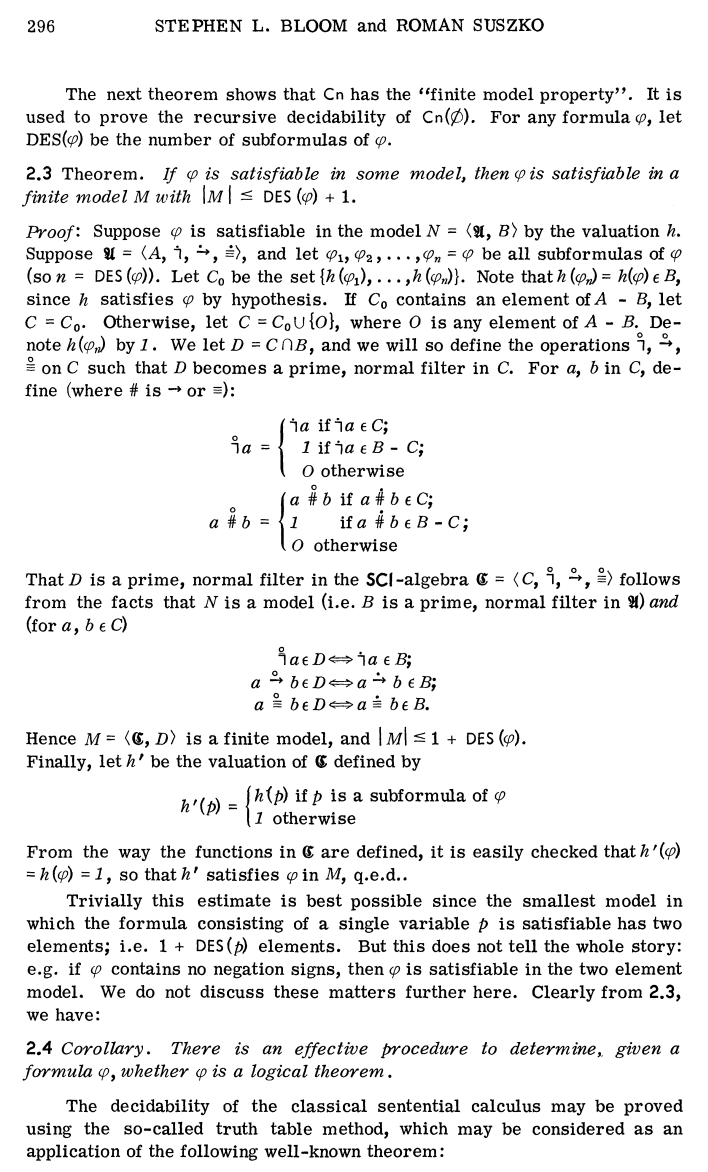
\includegraphics[scale=0.65]{Suszko.png}

\subsection*{Translacja symboli Suszki}

\begin{tabular}{ |c|c| }
  \hline
  Suszko       & moja notacja  \\
  \hline
  \textgoth{U} & $\mathcal{M}$ \\
  \hline
  $A$          & $U$           \\
  \hline
  $B$          & $D$           \\
  \hline
  $h $         & $V $          \\
  \hline
  $C $         & $U' $         \\
  \hline
  $D $         & $D' $         \\
  \hline
  $h' $        & $V' $         \\
  \hline
\end{tabular}

Definicja skończonego modelu:
\begin{itemize}
  \item $1 = V(\varphi), 0 = $ dowolny element z $U \setminus D$.
  \item $U' = \{V(\varphi_1), ..., V(\varphi_n) = 1, 0\}$ ($0 = $ pewne $ V(\varphi_i)$, jeśli tylko $\exists V(\varphi_i) \in U'\setminus D'$)
  \item $D' = U' \cap D$
  \item For $a \in U'$: $ \tilde{\lnot}'a = \begin{cases}
            \tilde{\lnot}a , & \text{if } \tilde{\lnot}a \in U'              \\
            1,               & \text{if } \tilde{\lnot} a \in D \setminus U' \\
            0,               & \text{otherwise }                             \\
          \end{cases}
        $
  \item $V'(\psi) = \begin{cases}
            V(\psi) , & \text{if } \psi \in \SUB(\varphi) \\
            1,        & \text{otherwise }
          \end{cases}$
\end{itemize}

\subsection*{Trywialny kontrprzykład}

$V'(\lnot \varphi) = 1$ -- z def $V'$, bo $\lnot \varphi \not \in \SUB(\varphi)$

$V'(\lnot \lnot \varphi) = 1$ -- z def $V'$, bo $\lnot \varphi \not \in \SUB(\varphi)$

Więc $V'$ to nie waluacja, bo nieprawda, że $V'(\lnot \psi) \in D$ iff
$V'(\psi) \not \in D$.

Ale to łatwo naprawić robiąc $V'(\psi) \in \{1, 0\}$ gdy $\psi \not \in
  \SUB(\varphi)$.

\subsection*{Poprawka i ogólny problem z definicją $V'(\psi)$ w stylu: $\psi \not \in SUB(\varphi) \Rightarrow V'(\psi) \in \{1, 0\}$}

$V'(\psi) = \begin{cases}
    V(\psi) , & \text{if } \psi \in \SUB(\varphi)        \\
    1,        & \text{otherwise, if } V(\psi) \in D      \\
    0,        & \text{otherwise, if } V(\psi) \not \in D \\
  \end{cases}$

Kontrprzykład, pokazujący że $V'$ nie jest waluacją:

Mamy dane:

\begin{itemize}
  \item $\varphi = \lnot(p \id \lnot p)$
  \item $U = \{a, b, c, d, ...\}$,
  \item $D = \{a, c, ...\}$,
  \item $V(\varphi) = a \in D$
  \item $V(p \id \lnot p) = b \not \in D$
  \item $V(p) = c \in D$
  \item $V(\lnot p) = d \in D$
  \item $V(\lnot \varphi) = b \not \in D$, $V(\lnot \lnot \varphi) = a \in D$, ...
  \item $\tilde{\lnot}a = b$, $\tilde{\lnot}b = a$
  \item $\tilde{\lnot}c = d$, $\tilde{\lnot}d = c$
\end{itemize}

\begin{tikzpicture}
  \begin{scope}[every node/.style={circle,draw}]
    \node (a) [very thick] at (0,0) {a};
    \node (b) at (0,3) {b};
    \node (d) at (2.5,3) {d};
    \node (c) [very thick] at (2.5,0) {c};
  \end{scope}

  \path [->] (a) edge[bend right] node {$\tilde{\lnot}$} (b);
  \path [->] (b) edge[bend right] node {$\tilde{\lnot}$} (a);
  \path [->] (c) edge[bend right] node {$\tilde{\lnot}$} (d);
  \path [->] (d) edge[bend right] node {$\tilde{\lnot}$} (c);
\end{tikzpicture}

Dostaniemy:
\begin{itemize}
  \item $U' = \{a, b, c, d\}$
  \item $D' = \{a, c\}$
  \item $1 = a$. Przyjmijmy $0 = d$
  \item $\tilde{\lnot}'a = b, \tilde{\lnot}'b = a$
  \item $V'(\varphi) = a$
  \item $V'(\lnot \varphi) = 0 = d$
  \item Więc $\tilde{\lnot}'V'(\varphi) = \tilde{\lnot}'a = b \not = 0 = V'(\lnot
          \varphi)$, więc $V'$ nie jest waluacją.
\end{itemize}

\subsection*{Próba prostej poprawki $V'$}

% $
%   \tilde{\lnot}'a = \begin{cases}
%     \tilde{\lnot}a , & \text{if } a \in U \text{ and } \tilde{\lnot}a \in U' \\
%     0,               & \text{otherwise, if } a \in D'                        \\
%     1,               & \text{otherwise, if } a \not \in D'                   \\
%   \end{cases}
% $

$V'(\psi) = \begin{cases}
    V(\psi) , & \text{if } V(\psi) \in U'                \\
    1,        & \text{otherwise, if } V(\psi) \in D      \\
    0,        & \text{otherwise, if } V(\psi) \not \in D \\
  \end{cases}$

Kontrprzykład, pokazujący że $V'$ nie jest waluacją:

Mamy dane:

\begin{itemize}
  \item $\varphi = \lnot(p \id \lnot p)$
  \item $U = \{a, b, c, d, z, ...\}$
  \item $D = \{a, c, ...\}$
  \item $\tilde{\lnot}a = z$, $\tilde{\lnot}z = a$
  \item $\tilde{\lnot}b = a$
  \item $\tilde{\lnot}c = d$, $\tilde{\lnot}d = c$
  \item $V(p) = c, V(\lnot p) = d, V(p \id \lnot p) = b$
  \item $V(\varphi) = a$
  \item $V(\lnot \varphi) = z$
  \item $V(\lnot \lnot \varphi) = a$
\end{itemize}

\begin{tikzpicture}
  \begin{scope}[every node/.style={circle,draw}]
    \node (a) [very thick] at (0,0) {a};
    \node (z) at (-2.5,1) {z};
    \node (b) at (0,3) {b};
    \node (c) [very thick] at (2.5,0) {c};
    \node (d) at (2.5,3) {d};
  \end{scope}

  \path [->] (a) edge[bend right] node {$\tilde{\lnot}$} (z);
  \path [->] (z) edge[bend right] node {$\tilde{\lnot}$} (a);
  \path [->] (b) edge[bend right] node {$\tilde{\lnot}$} (a);
  \path [->] (c) edge[bend right] node {$\tilde{\lnot}$} (d);
  \path [->] (d) edge[bend right] node {$\tilde{\lnot}$} (c);
\end{tikzpicture}

I dostajemy:
\begin{itemize}
  \item $U' = \{a, b, c, d\}$
  \item $D = \{a, c \}$
  \item $1 = a$
  \item Weźmy, że $0 = d$
  \item $\tilde{\lnot}'b = a$
  \item $\tilde{\lnot}'a = 0 = d$
  \item $\tilde{\lnot}'d = c$
  \item $\tilde{\lnot}'c = d$
        \begin{tikzpicture}
          \begin{scope}[every node/.style={circle,draw}]
            \node (a) [very thick] at (0,0) {a};
            \node (b) at (0,3) {b};
            \node (c) [very thick] at (2.5,0) {c};
            \node (d) at (2.5,3) {d};
          \end{scope}

          \path [->] (a) edge[bend right] node {$\tilde{\lnot}$} (d);
          \path [->] (b) edge[bend right] node {$\tilde{\lnot}$} (a);
          \path [->] (c) edge[bend right] node {$\tilde{\lnot}$} (d);
          \path [->] (d) edge[bend right] node {$\tilde{\lnot}$} (c);
        \end{tikzpicture}
  \item $V'(\varphi) = a$
  \item $V'(\lnot \varphi) = 0 = d$
  \item $V'(\lnot \lnot \varphi) = a$
  \item I dostajemy: $\tilde{\lnot}'V'(\lnot \varphi) = \tilde{\lnot}' 0 = 1 = c$
  \item Ale: $V'(\lnot \lnot \varphi) = a$, więc $\tilde{\lnot}'V'(\lnot \varphi) \not
          = V'(\lnot \lnot \varphi)$, więc $V'$ nie jest wartościowaniem.
\end{itemize}

\subsection*{Druga próba poprawki $V'$}

$V'(\psi) = \begin{cases}
    V(\psi) ,                          & \text{if } \psi \in \SUB(\varphi)'              \\
    1,                                 & \text{otherwise, if } \psi = p \in D            \\
    0,                                 & \text{otherwise, if } \psi = p \not \in D       \\
    \tilde{\lnot}'V'(\vartheta),       & \text{otherwise, if } \psi = \lnot \vartheta    \\
    V'(\vartheta)\tilde{\ra}'V'(\chi), & \text{otherwise, if } \psi = \vartheta \ra \chi \\
    V'(\vartheta)\tilde{\id}'V'(\chi), & \text{otherwise, if } \psi = \vartheta \id \chi \\
  \end{cases}$

Chodzi o to, że $V'$ jest zdefiniowane indukcyjnie, po $s(\psi)$, korzystając z $V'$ dla mniejszych $\psi$.

Widać, że:
\begin{itemize}
  \item $V'(\psi) \in U'$
  \item $\tilde{\lnot}'V'(\psi) = V'(\lnot \psi)$
\end{itemize}

\end{document}